%\section{Diseño Estructural y Especificaciones de Diseño}

\subsubsection{Descripción General del Sistema}

El sistema robótico diseñado para la manipulación automatizada de lechugas en cultivos hidropónicos verticales presenta una configuración cartesiana de dos ejes (XZ), con dimensiones de 3~m de ancho por 2~m de alto. El robot está equipado con un brazo robótico serie que posee un efector final tipo pinza con dos grados de libertad para la sujeción y traslado de las lechugas.

\subsubsection{Configuración Estructural}

El diseño estructural se basa en dos subsistemas de movimiento perpendiculares, cada uno optimizado según los requerimientos de carga y precisión:

El eje horizontal implementa un sistema de transmisión por correa dentada y poleas, accionado mediante motor paso a paso. La característica distintiva de este diseño es que la carga móvil se soporta mediante un perfil tipo poli-V equipado con ruedas de desplazamiento. Esta configuración permite que la correa de transmisión trabaje prácticamente sin carga de peso, funcionando únicamente como elemento de tracción, lo cual mejora significativamente la precisión del posicionamiento y reduce el desgaste del sistema.

El conjunto incluye un tensor de correa ajustable que mantiene la tensión óptima durante la operación, compensando elongaciones del material y garantizando transmisión sin deslizamiento. Además cuenta con un perfil guia, en el lateral del suporte superior, paralelo al perfil de soporte superior. Esto da rigidez lateral al sistema y anula la oscilación alrededor del perfil horizontal.

\begin{figure}[H]
    \centering
    \begin{subfigure}{0.35\textwidth}
        \centering
        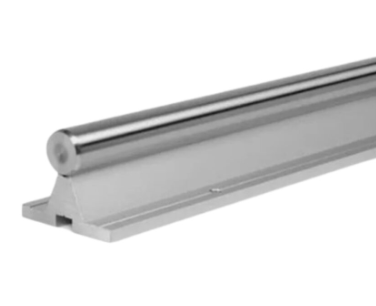
\includegraphics[width=\textwidth]{img/barra_lateral.png}
        \caption{Barra lateral.}
        \label{fig:barra_lateral}
    \end{subfigure}
    \hfill
    \begin{subfigure}{0.3\textwidth}
        \centering
        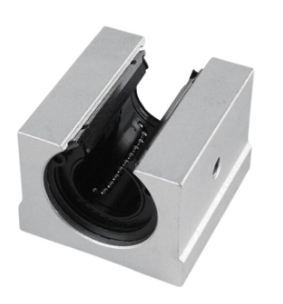
\includegraphics[width=\textwidth]{img/sbr20uu.png}
        \caption{Carro para deslizamiento sobre barra lateral.}
        \label{fig:sbr20uu}
    \end{subfigure}
    \caption{Sistema de rigidez horizontal.}
\end{figure}

El movimiento vertical se realiza mediante transmisión por tornillo de potencia, proporcionando capacidad de carga superior y autobloqueo mecánico. Para garantizar la rigidez del sistema y evitar rotaciones indeseadas del carro móvil, se incorporan dos varillas lisas de acero dispuestas en paralelo a la varilla roscada. Esta configuración de tres varillas paralelas asegura un movimiento vertical estable y preciso: la varilla roscada transmite el movimiento mientras que las dos varillas lisas actúan como guías lineales, proporcionando rigidez lateral y evitando giros del soporte, especialmente bajo cargas asimétricas.

Por otro lado, el robot cuenta con tres soportes estructurales principales fabricados mediante impresión 3D:

\begin{itemize}
    \item \textbf{Soporte inferior:} Fijación de las varillas verticales y montaje del motor del eje Z
    \item \textbf{Soporte superior:} Permite el acoplamiento cinemático de los dos movimientos perpendiculares (horizontal y vertical), actuando como elemento de unión entre ambos subsistemas
    \item \textbf{Soporte medio:} Sostiene el brazo robótico y la cámara y se mueve cuando gira la varilla.
\end{itemize}

\subsubsection{Cargas del Sistema}

Las cargas consideradas en el diseño se distribuyen según su función operativa:

\paragraph{Cargas del eje horizontal:}
Es la suma del peso de las varillas, la varilla roscada, la carga, los soportes y el brazo. Considerando que aproximademente toda la carga la sostiene el perfil superior, se tiene que la carga aproximada que debe mover el motor es de aproximadamente 2kg
%\begin{itemize}
%    \item Carga a mover por el motor en horizontal: 2~kg
 %   \item Peso de varillas lisas (guías verticales): 1.578~kg cada una (6.312~kg total para 4 varillas)
  %  \item Peso de varilla roscada: 1.208~kg cada una (2.416~kg total para 2 varillas)
   % \item Peso de soportes estructurales: 4~kg
%\end{itemize}

\paragraph{Cargas del eje vertical:}
Es la suma del peso de la lechuga y el brazo. Además el motor debe vencer la fricción que se genera entre la tuerca y la varilla.

\subsubsection{Especificaciones Cinemáticas}

Las especificaciones de velocidad, aceleración y resolución de los actuadores se detallan en la Tabla~\ref{tab:especificaciones_cinematicas}.

\begin{table}[htbp]
\centering
\caption{Especificaciones cinemáticas de los ejes de movimiento}
\label{tab:especificaciones_cinematicas}
\begin{tabular}{|l|c|c|}
\hline
\textbf{Parámetro} & \textbf{Eje Horizontal} & \textbf{Eje Vertical} \\ \hline
Velocidad máxima [\(\frac{mm}{s}\)] & 250 & 75 \\ \hline
Velocidad mínima [\(\frac{mm}{s}\)] & 12.5 & 2.5 \\ \hline
Aceleración [\(\frac{mm}{s^2}\)] & 187.5 & 45 \\ \hline
Avance por revolución [\(\frac{mm}{rev}\)] & 40 & 8 \\ \hline
Resolución [\(\frac{pasos}{mm}\)] & 40 & 200 \\ \hline
Micropasos & 8 & 8 \\ \hline
\multicolumn{3}{c}{} \\
\end{tabular}
\end{table}

La diferencia en resolución entre ambos ejes responde a los requisitos operativos: el eje horizontal requiere mayor velocidad de desplazamiento con precisión moderada, mientras que el eje vertical necesita mayor precisión de posicionamiento con velocidades menores debido a las operaciones de elevación de carga.